\documentclass{article}

\usepackage[margin=0.75in, headheight=35pt, includehead, includefoot]{geometry}

\usepackage{fancyhdr}
\usepackage[T1]{fontenc}
\usepackage[shortlabels]{enumitem}
\usepackage{graphicx}
\graphicspath{ {./} }
\usepackage[export]{adjustbox}
\usepackage{booktabs}
\usepackage{forest}
\usepackage{listings}
\lstset{escapeinside={(*@}{@*)}}

\setlength{\parindent}{4em}
\setlength{\parskip}{1em}

\pagestyle{fancy}
\rhead{Alex Kitsul\\230134210\\February 16, 2021}

\begin{document}
\thispagestyle{empty}
\begin{center}
\topskip0pt
\vspace*{\fill}
\Huge Alex Kitsul\\
\Huge 230134210\\
\Huge CPSC 450\\
\Huge Assignment 3 - Report\\
\Huge February 16\\
\vspace*{\fill}
\end{center}
\pagebreak

\section*{Psedocode}
\begin{lstlisting}
main:
	string1 <- from file
	string2 <- from file
	
	table <- make_table(string1, string2)
	lcs <- LCS(table, string1, string2, len(string0), len(string1))
	lcs_all <- LCS_All(table, string1, string2, len(string0), len(string1))
	
	display lcs
	display lcs_all
	
make_table(string1, string2):
	table = height[len(string2) + 1], width[len(string1) + 1]
	table <- all values set to 0
	
	for i from 1 to table width:
		for j from 1 to table height:
			if string1[i - 1] == string2[j - 1]:
				table[i][j] = table [i - 1][j - 1] + 1
			else:
				table[i][j] = max(table[i][j - 1], table[i - 1][j])
				
	return table
			
LCS(table, string1, string2, i, j):
	if (i or j == 0):
		return ""
		
	if (string1[i - 1] == string2[j - 1]):
		return LCS(table, string1, string2, i - 1, j - 1) + string1[i - 1]
		
	if (table[i][j - 1] > table[i - 1][j]):
		return LCS(table, string1, string2, i, j - 1)
		
	return LCS(table, string1, string2, i - 1, j)
	
LCS_All(table, string1, string2, i, j):
	if (i or j == 0):
		return [""]
		
	if (string1[i - 1] == string2[j - 1]):
		lcs = LCS_All(table, string1, string2, i - 1, j - 1)
		
		for k in len(lcs):
			lcs[k] = lcs[k] + string1[i - 1]
			
		return lcs
		
	list <- []
		
	if (table[i][j - 1] >= table[i - 1][j]):
		list = LCS_All(table, string1, string2, i, j - 1)
		
	if (table[i - 1][j] >= table[i][j - 1]):
		list = list + LCS_All(table, string1, string2, i, j - 1)
		
	return list
		
\end{lstlisting}

\pagebreak

\section*{Program Code}
\textbf{\underline{LCS.py}}
\begin{lstlisting}
def main():
    """
        Main driver method

        Parameters:

            None

        Returns:

            None. Side effect.
    """
    file_input = input("Enter file name: ")

    with open(file_input, "r") as file:
        string = file.read()
        string = string.split("\n")

        table = make_table(string[0], string[1])
        print("One LCS value: ", LCS(table, string[0], string[1], len(string[0]),
        	len(string[1])))
        print("All possible LCS values: ", LCS_all(table, string[0], string[1],
         	len(string[0]), len(string[1])))

def make_table(string1, string2):
    """
        Makes the DP Table and fills in values

        Parameters:

            string1 (String): First string
            string2 (String): Second string

        Returns:

            table (list[list[int]]): Dynamic programming 2D table
    """

    # Initialize all values to 0
    table = [[0 for row in range(len(string2) + 1)]
    		for col in range(len(string1) + 1)]

    # Populate the count of each character in the order for both strings
    for i in range(1, len(string1) + 1):
        for j in range(1, len(string2) + 1):
            if (string1[i - 1] == string2[j - 1]):
                table[i][j] = table[i - 1][j - 1] + 1
            else:
                table[i][j] = max(table[i][j - 1], table[i - 1][j])

    return table

def LCS(table, string1, string2, i, j):
    """
        Takes the DP Table and bracktracks out a Longest Common Sequence

        Parameters:

            table (list[list[int]]): DP Table
            string1 (String): First string
            string2 (String): Second string
            i (int): current x location in DP table
            j (int): current y location in DP table

        Returns:

            lcs (String): Longest common sequence
    """
    # Finished backtracking
    if (i == 0 or j == 0):
        return ""

    # If both values are equal, go diagonal
    if (string1[i - 1] == string2[j - 1]):
        return LCS(table, string1, string2, i - 1, j - 1) + string1[i - 1]

    # If the value above is greater, move up
    if (table[i][j - 1] > table[i - 1][j]):
        return LCS(table, string1, string2, i, j - 1)

    # If the value left is greater, go left
    return LCS(table, string1, string2, i - 1, j)

def LCS_all(table, string1, string2, i, j):
    """
        Takes the DP Table and bracktracks out all 
        possible longest common sequences

        Parameters:

            table (list[list[int]]): DP Table
            string1 (String): First string
            string2 (String): Second string
            i (int): current x location in DP table
            j (int): current y location in DP table

        Returns:

            lcs (list[String]): Longest common sequence
    """
    # Finished backtracking
    if (i == 0 or j == 0):
        return [""]

    # If both values are equal, go diagonal
    if (string1[i - 1] == string2[j - 1]):
        lcs = LCS_all(table, string1, string2, i - 1, j - 1)

        for k in range(len(lcs)):
            lcs[k] = lcs[k] + string1[i - 1]

        return lcs

    # Define empty list to be added to
    list = []

    # If the value above is greater, backtrack from there
    if (table[i][j - 1] >= table[i - 1][j]):
        list = LCS_all(table, string1, string2, i, j - 1)

    # If the value to the left is greater, backtrack from there
    if (table[i - 1][j] >= table[i][j - 1]):
        list = list + LCS_all(table, string1, string2, i - 1, j)

    return list

if __name__ == "__main__":
    main()

\end{lstlisting}

\pagebreak

\section*{Examples with Output}
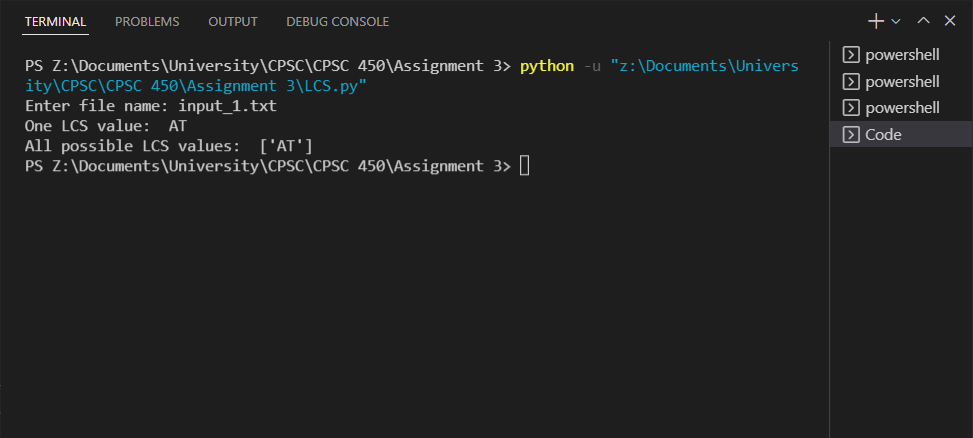
\includegraphics[scale=0.5]{ExampleInput1.png}\\
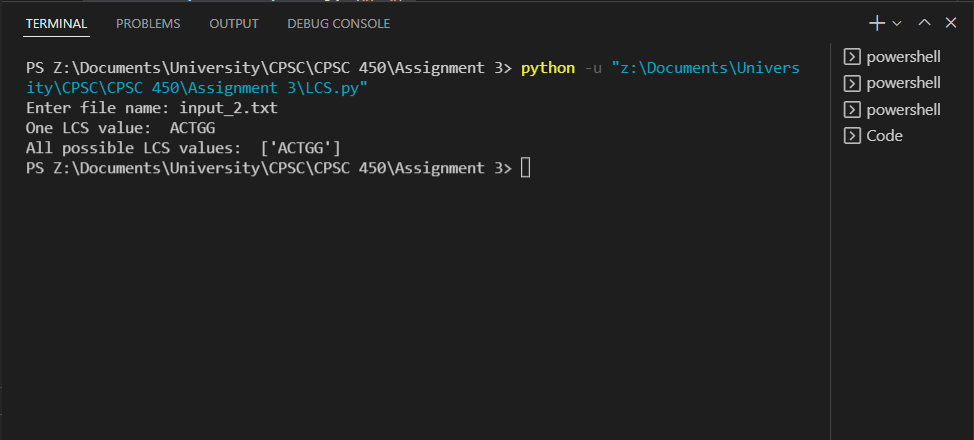
\includegraphics[scale=0.5]{ExampleInput2.png}\\
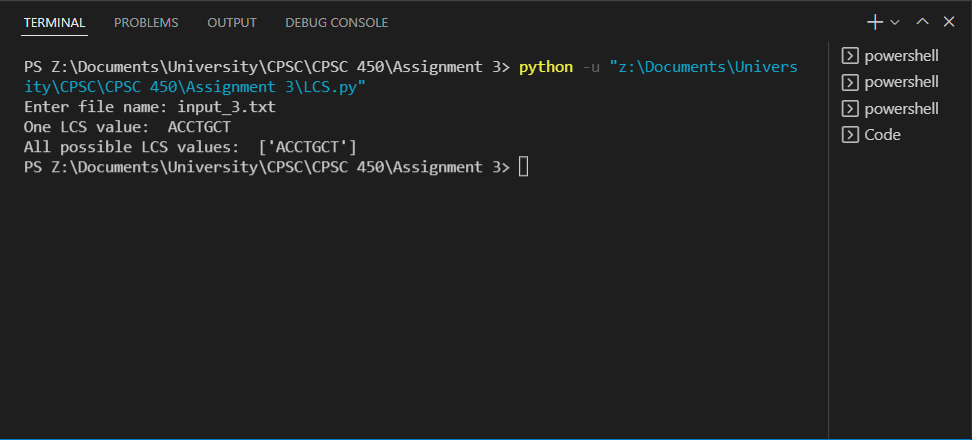
\includegraphics[scale=0.5]{ExampleInput3.png}\\

\end{document}
